\section{Meddle Overview}

In this section, we present an overview of \meddle. We first describe the goals and non-goals of the 
system, then present the \meddle architecture. We evaluate the performance of our system and discuss 
the current deployment.

\subsection{Goals}

The goals of our system are to provide visibility into Internet traffic from mobile devices, 
exert control over this traffic and facilitate a large deployment across multiple 
networks, OSes and devices. We discuss each of these in turn.

\begin{packeditemize}
\item \emph{Visibility}. One of our goals is to capture all of a mobile-device's Internet traffic all of the time, 
allowing us to characterize network flows and interpose on them using software middleboxes. Thus, 
we need a solution that works continuously over time, regardless of the device OS, network, 
access technology, device or apps installed. Our VPN-based proxy achieves these goals. Further, 
as network flows are increasingly encrypted, we lose the ability to interpose on the corresponding 
traffic. To address this problem, we propose a limited use of SSL-bumping (enabled by the user) 
that allows us to decrypt, inspect and modify encrypted traffic (\eg to strip out PII).
  
\item \emph{Control}. Another important goal is to facilitate research into new middlebox approaches 
for interposing on mobile Internet traffic. The system must support the ability to deploy and distribute large numbers 
of middlebox services quickly, easily and at scale~\cite{sherry:middleboxes} without 
the need to deploy hardware in homes~\cite{bismarck} or ISPs~\cite{wang:middleboxes}. 
It should present a simple API for researchers and developers to block, shape, inject or otherwise 
modify network flows, and it should support services to improve network performance, security, 
privacy and efficiency. 

\item \emph{Deployable}. Our system can facilitate experiments in a lab environment and using naturally 
user-generated flows ``in the wild''. To support the latter, we need a system that has incentives for users, 
a low barrier to adoption, is easy to deploy and that scale gracefully. 
  
\end{packeditemize}
  

\subsection{Design}

In this section, we describe the design and implementation of \meddle and describe how 
it meets the goals described in the previous section.

At a high level, \meddle is a system consisting of one or more servers that interact with a 
mobile device's Internet traffic. Primarily, \meddle uses a VPN tunnel to directs all of a 
mobile device's naturally generated Internet traffic to a proxy server, which we call a \meddlebox. 
Section~\ref{subsec:design_visibility} describes how this achieves our goal of visibility.

Once traffic arrives at the \meddlebox, we can record, block, modify and/or otherwise interact 
with mobile-device Internet traffic. Section~\ref{subsec:design_control} discusses how we 
use software middlebox techniques to achieve our goal of controlling mobile-device traffic. 

A key advantage of \meddle is that it provides a platform for experimenting 
with new and existing services that interact with user-generated traffic (\ie ``in the wild''). 
To access this user-generated traffic, we need to convince users to participate in the system. 
Section~\ref{subsec:design_deploy} describes how we designed \meddle to have clear 
incentives for user adoption, a low barrier to entry to participate, and good performance that 
is easy to scale to a global deployment.

TODO insert new figure 

\begin{figure}[h]
\centering
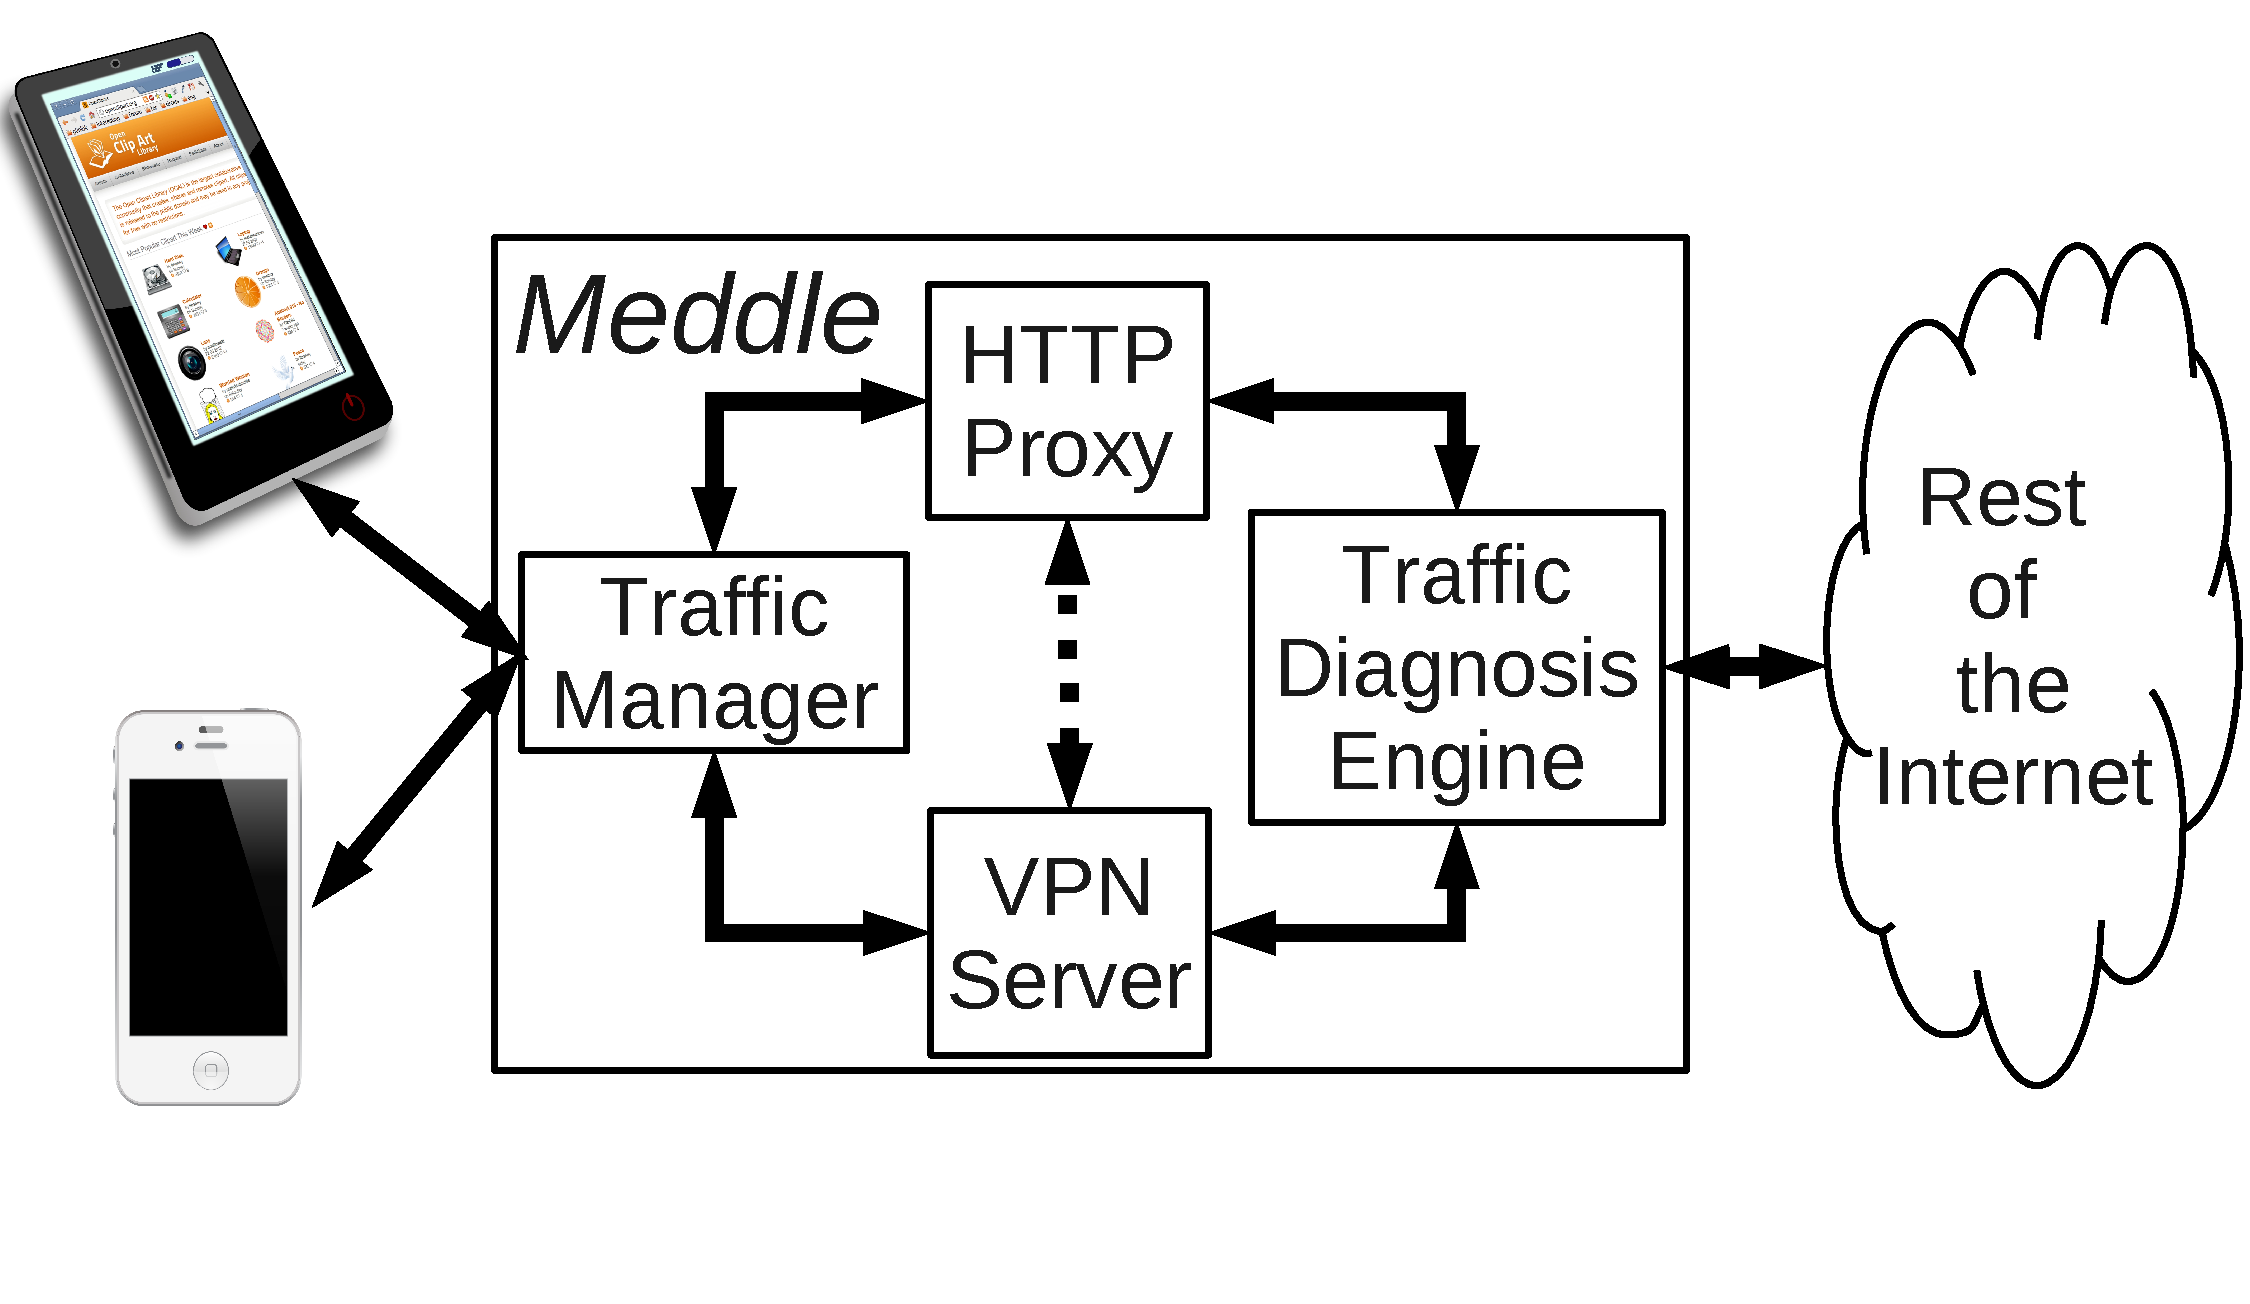
\includegraphics[width=\columnwidth]{figures/Meddle-Design.pdf}
\caption{Traffic diagnosis using VPN and HTTP proxy based traffic redirection.}
\label{fig:architecture}
\end{figure}

%%%%%%%

%\meddle attains its goals by exploiting the observation that nearly all devices support network traffic indirection via virtual private networks (VPNs) and HTTP proxies. 
%This network perspective offered by traffic redirection is promising because mobile devices are increasingly becoming the primary gateway to access Internet based services~\cite{ict:facts}. 
%This perspective becomes even more important because a large number of free applications use Internet connectivity with the sole purpose of serving advertisements that make-up for their costs~\cite{pathak:eprof,vallina-rodriguez:bfc}.
%
%
%As depicted in Figure~\ref{fig:architecture}, \meddle relies on a combination of VPN and HTTP based proxies to diagnose traffic from mobile apps and OS services, and to identify ISP interference.
%\meddle uses HTTP proxies, that exchange traffic in the clear, to identify possible ISP interference with HTTP traffic. 
%\meddle uses VPNs to address potential ISP interference, and to diagnose the traffic naturally generated by the mobile apps and OS services.
%
%\meddle's traffic manager determines the flow of the packet, through a combination of VPN and HTTP proxies, before the packet enters the traffic diagnosis engine. 
%On this engine, we deploy a variety of diagnosis tools such as bro. 
%\tbd{Here it must be highlighted that \meddle allows the integration of the existing tools to offer a single platform that can be used for mobile traffic diagnosis. Though simple, it brings with it a power that previously required warranty voiding of devices and ... The novelty lies in exploiting existing features to come up with a feasible user friendly platform}
%
%
%
%VPNs are supported by most mobile OSes\footnote{Android, BlackBerry, and iOS all support VPNs natively, representing more than 86\% of the mobile device market\cite{gartner-phone-share}.} and carriers to satisfy their enterprise clients. 
%Thus \meddle leverages on VPNs for being agnostic to mobile OSes, ISPs, access technologies, and applications used by the mobile device.
%\tbd{what about other goals.. I do not want to put a see section .. here.}
%
%%\subsubsection{Architecture}
%
%\meddle uses VPNs as a portable mechanism to tunnel traffic from mobile devices to a machine outside of the carrier's network for the purpose of analysis and interposition.
%\meddle uses the Squid~\cite{squid} HTTP proxy for two purposes: 1) to monitor the SSL traffic using SSL bumping~\cite{sslbump} which is essentially a man-in-the-middle operation, and 2) inject javascript code inspired by tripwires~\cite{tripwires} to identify ISP interference.
%
%\meddle currently offers the following capabilities to diagnose mobile Internet traffic
%\begin{packedenumerate}
%\item Passive monitoring to characterize the network behavior of application and OS services. 
%\item Enhanced passive monitoring to analyze SSL traffic.
%\item Analysis of ISP interference.
%\item Filtering privacy invasive traffic. 
%\end{packedenumerate}

\subsubsection{Visibility into Mobile Internet Traffic}
\label{subsec:design_visibility}

\meddle leverages the fact that the vast majority of mobile devices provide native VPN support, a feature typically provided to satisfy enterprise clients. We currently support VPN tunnels on iOS and Android; we anticipate being able to support the next version of Windows Phone that includes a native VPN implementation.

\noindent\textbf{iPhone support.} 
All iOS devices (version 3.0 and above) support \textit{VPN On-Demand}, which forces traffic for a specified set of domains to use VPN tunnels. 
This feature is originally intended to allow enterprises to ensure their employees' devices always establish a VPN connection before contacting a specified set of domains. 
To ensure all possible destinations match this list, we exploit the fact that iOS uses suffix matching to determine which connections should be tunneled; accordingly, we specified the domain list as the set of alphanumeric characters (a-z, 0-9, one character per domain). 
To setup this configuration, users need to install a single file, a step that needs to be performed only once. 

\noindent\textbf{Android support.} As of Android 4.2, Android supports ``always on'' VPN connections that ensure all traffic is always tunneled.
For Android version 4.0 and above there is an app API that allows apps to manage VPN tunnels. 
We use this API in the StrongSwan implementation of a VPN client~\cite{strongswanclient} that ensures re-establishment of VPN tunnels on network state changes (\eg, when a device switches from cellular to \wifi).
\meddle thus supports devices running Android version 4.0 and above.

\noindent\textbf{Server-side implementation.} 
\meddle uses the free and open-source Strongswan~\cite{strongswan} to manage the VPN tunnels 
on its servers. When traffic arrives at the server, we use \emph{tcpdump} and \emph{bro} to record 
traffic. We use two IRB-approved measurement approaches. One approach captures full packets, 
and requires subjects to be interviewed and provide written informed consent before participating. 
We used this study to inform the second approach, which captures only relevant packet headers 
necessary for the applications we discuss in the remainder in the paper. 

As we described in the previous section, encrypted flows gives \meddle no visibility into the 
content of network flows and no ability interpose on that traffic. To regain this visibility, we use SSL 
bumping to decrypt and access the plaintext of encrypted flows in the following way. 
 
First, we note that \meddle's VPN server, like all VPN servers, can be configured to use self-generated root certificate used to sign all subsequent certificates issued to participating mobile devices. 
This allows us to perform SSL traffic decryption using the Squid proxy's SSL bumping~\cite{sslbump} feature.
When the mobile device connects to a services supporting SSL, the proxy masquerades as the service using a forged certificate signed with the \meddle root certificate. 
Then the proxy establishes an SSL connection with the intended target, impersonating a mobile device. 
Using the traffic captured on \meddle and the private key generated by the squid proxy to communicate with the mobile device, we can decrypt all SSL traffic. We note that when traffic is not encrypted using SSL, the proxy simply forwards traffic. 

This approach fails for apps that do not trust certificates signed by unknown root authorities. 
For example, in our controlled experiments we observed that Firefox prevents SSL bumping by validating root certificates, while the Google Chrome, Safari, Facebook, and Google+ apps, as well as the default mail clients and advertisement services, do not check the validity of the root certificate. 
This enables our approach to provide visibility into secure channels established with a wide range of popular apps. 

Currently we use this only in controlled experiments 
where \emph{no user traffic is intercepted}. We are also designing a study for IRB approval where we 
will use SSL bumping to remove PII from user-generated traffic only when users opt in.

\subsubsection{Services for Controlling Traffic}
\label{subsec:design_control}
\begin{figure}
\begin{center}
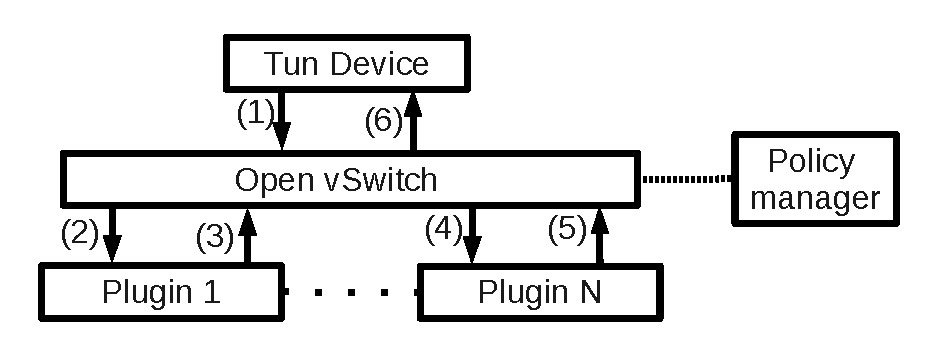
\includegraphics[width=\columnwidth]{figures/packet-monitoring-plugin.pdf}
\end{center}
\caption{Plugin Infrastructure on \platname.}
\label{fig:packet-monitoring-solution}
\end{figure}

Once traffic arrives at a \meddlebox, it interacts with one or more 
services. These consist of software middleboxes that interpose on 
user-generated traffic, which are accessed 
via a plugin infrastructure, and proxy services that interact with 
flows that \meddle induces.  

\noindent\textbf{Plugin infrastructure.} Figure~\ref{fig:packet-monitoring-solution} shows how 
\platname{} supports a plugin
infrastructure for custom flow processing. Each plugin takes as input a 
network flow and outputs a network flow (potentially empty). 
When a packet is received at the TUN
device, it is sent to a software-defined switch~\cite{Openvswitch} that 
determines the ordered set of plugins that flows will traverse. 
This order is configured by a policy manager, which determines 
the set of plugins that should operate on each flow. After the last 
plugin is traversed, the network flow is sent out through the TUN device 
to the Internet. 

Plugins support a variety of features such as ad blocking, 
analyzing PII leakage or page speed optimization. We 
 use a plugin to enable SSL traffic decryption (described in the previous section) using 
the \platname{} plugin infrastructure. Additionally, we have implemented 
per-connection blocking, malware analysis and DNS-based packet filters. 

\noindent\textbf{Proxy services.} As we describe in Section~\ref{}, we can use 
\meddle to conduct active measurements. 
Specifically, we currently inject JavaScript into Web pages to detect if the device's 
access network is modifying Web content in flight, and we use a companion app to 
test detect service differentiation within mobile ISPs. To support these services, we 
run services on \meddle servers that are accessed via untunneled connections. 

\subsubsection{Deployability}
\label{subsec:design_deploy}

This section describes how \meddle provides clear incentives for user adoption, a 
low barrier to entry and reasonable performance that is easy to scale.

\noindent \textbf{Incentives for user adoption.} \meddle presents a number of incentives 
that appeal to a wide range of users. Importantly, we do not charge users for any of these 
services.

\begin{packeditemize}
\item \emph{Improved security.} By securely tunneling all of a mobile device's traffic, users 
are less vulnerable to data leakage (\eg via open WiFi hotspots). 
\item \emph{Device-wide content filters.} We use \meddle to block content that users do 
not wish to access -- for all apps running on a device. The most popular instance of this is 
device-wide ad blocking.
\item \emph{Privacy revelations.} The \emph{ReCon} tool allows users to see how they are being 
tracked by ad and analytic servers, and allows them to create per-connection block lists.  
\item \emph{Malware detection.} \meddle uses network signatures to identify malware, block it from 
communicating and prevent future downloads onto other \meddle-enabled devices.  
\item \emph{ISP transparency.} We provide services that allow users to identify cases where 
ISPs are modifying HTTP content in flight, and when they provide differentiated service to 
traffic crossing their networks.
\end{packeditemize}

\noindent \textbf{Low barrier to entry.} 
Manually configuring a VPN generally requires filling out five fields on an Android phone, and the VPN configuration can be distributed using a single file on iOS. 
These configurations are primarily required to drive the key exchange algorithms required to establish the VPN tunnels.

Our \meddlebox system requires only that the user can run a modern Linux OS with root privileges. This can be deployed 
in a single-machine instance on a home computer, dedicated server or on a VM in the cloud. \meddle is currently in private beta with dedicated-server, EC2 and Aliyun deployments in the US, France and China. We will make the \meddle software publicly available.

\noindent \textbf{Performance and Scalabilty.} 

\noindent\emph{Network Latency.}
We measured 50 VPN-connection establishment times  on both iOS (iPhone 5 / iOS 6.1) and Android (Galaxy Nexus /
Android 4.2), for \wifi{} and cellular connections. 
The \meddle server was running on a university network. 
For Android (using IKEv2), the maximum establishment time was 0.81 seconds on \wifi{} and 1.59 seconds on cellular. 
For iOS (using IKEv1), the connection takes longer due to the older protocol version: we observe a maximum of 2 seconds on \wifi{} and 2.18 seconds on cellular. 
Because each VPN session supports many flows, the amortized cost of connecting is  small. 
\tbd{Cite results from latency to home gateways based on DSL results in PAM and IMC.}
\tbd{Address comments in conext review on latency}

\noindent\emph{Power Consumption.}
Mobile devices expend additional power to establish, maintain and encrypt data for a VPN tunnel. 
To evaluate the impact on battery, we used a power meter to measure the draw from a Galaxy Nexus running Android 4.2. 
We run 10-minute experiments with and without the VPN enabled. 
For each experiment, we used an activity script that included Web and map searches, Facebook interaction, e-mail and video
streaming. 
The VPN leads to a 10\% power overhead. \tbd{min, max, median for results given by dave}. 
For iOS devices, we relied on the battery readings provided by iOS because we cannot attach a power meter directly to the battery.
We again found an approximately 10\% power overhead of using VPNs when we drained a fully charged battery while performing the operations performed during the tests for Android devices.  

%\item 
\noindent\emph{Traffic Volume.}
\meddle relies on IPsec for datagram encryption, thus there is an encapsulation overhead for each tunneled packet. 
To evaluate this overhead, we use 30 days of data from 25 devices that to compare encapsulated and raw packet sizes. 
We observe a maximum encapsulation overhead of 12.8\% (average approximately 10\%). 
For users that have limited data plans and consume most of their quota per month, this can have 
a significant impact. We note that this is partially offset by \meddle services such as content filtering, 
connection blocking and optimizations such as transcoding and compression. 

\noindent\emph{Scalability.} We currently use Amazon EC2 to support users outside of China.\footnote{China 
blocks VPN access to all but domestic destinations; thus, we use a Chinese cloud host (Aliyun) to run  
\meddle in China.} Without exploring opportunities for economies of scale, we estimate that 
it will cost less than a penny (\$0.0084) per user per day. At this cost, we can support up to 
10,000 users with research funds. If \meddle were to become extraordinarily popular, it would 
cost each user approximately a quarter per month to pay their own way. By comparison, 
data plans in the US tend to cost \$30-\$90 per month -- more than two orders of magnitude larger.

%\end{packedenumerate}

\subsection{Generalizability and Limitations}

\noindent \textbf{Generalizability.} A system for improving visibility and control over Internet traffic from mobile 
devices can be implemented at the endpoints (\eg in the OS), in the network (\eg a hardware middlebox), 
somewhere else in the middle (our approach). \meddle is not intended as a blanket replacement for 
these alternative approaches; rather it allows us to explore the opportunities for improving the state of the 
art in today's mobile systems by making mobile Internet traffic available to researchers. 

In some cases, \meddle is the right location to implement new services that could be costly 
to deploy on devices (prefetching) or impractical to deploy in network (detecting ISP service differentiation). 
In other cases, \meddle provides a practical partial solution to a problem where the complete solution has an impractical 
cost. For example, identifying privacy leaks from mobile devices is reliably addressed using information flow 
analysis~\cite{taintdroid}. However, due to the overheads of this approach it is difficult to deploy to users 
and at scale. \meddle allows us to identify and block unobfuscated PII in network flows from arbitrary devices without requiring 
OS modifications or taint tracking. Regardless of the ultimate optimal solution, we can use \meddle today to inform the design 
and deployment of future functionality in OSes and for in-network devices. 

\noindent \textbf{Limitations.} The following technical limitations can impact \meddle's coverage.

\begin{packeditemize} 
\item\emph{At most one VPN tunnel.}
Currently iOS and Android support exactly one VPN connection at a time. 
This allows \meddle to measure traffic over either \wifi or cellular interfaces, but not both at once.
The vast majority of traffic uses only one of these interfaces, and VPNs can be used to tunnel that traffic.
\tbd{MPTCP on iOS 7??}

\item\emph{Proxy location.} 
When traffic traverses \meddle, destinations will see the \meddle box address, not the device IP, as the source. 
This might impact services  that customize (or block access to) content according to IP address (e.g., in case of localization). 
A solution to this problem is to use a \meddle{} instance with an appropriate IP address

\item\emph{ISP support.}
Some ISPs block VPN traffic, which prevents access to our current \meddle implementation. 
We note that few ISPs block VPN traffic, and there is an incentive not to block VPN traffic to support enterprise clients.

\item\emph{IPv6.}
\meddle{} cannot be currently used on networks using IPv6 because IPv6 is not fully supported by mobile devices. 
Indeed, we observe that though iOS and Android support IPv6 they currently do not support IPv6 traffic through VPN tunnels
\end{packeditemize} 


%\noindent\item \textbf{Wi-Fi Gateways powered by Cellular Modems.}


%\subsection{Costs}
%
%\noindent\textbf{Deployment and Running Costs}
%
%\noindent\textbf{Trust Provider}
%
%\subsection{Incentive for Deployment}
%
%\noindent \textbf{Deploy on Home Gateway.}
%This is why we need the single machine constraint. 
%
%\noindent \textbf{Packet Filtering.}
%Custom ad blocks. Protect against data leaks. 
%
%\noindent \textbf{User Interface to Packet Filtering.}
%
%\noindent \textbf{Security from untrusted Wi-Fi APs.}
%
%\subsection{Current Deployment}
%
%\footnote{\meddle is currently in private beta with deployments in the US, France and China. Users sign-up for an IRB approved study through \url{http://meddle.mobi}. We will make the \meddle software publicly available.} 
%
%\subsection{Discussion}




%\noindent \textbf{Modular Architecture for Offloading Activities.}



%%% Local Variables: 
%%% mode: latex
%%% TeX-master: "meddle-main"
%%% End: 
